% Section 9.3 (part of 09-performance.tex). Owner: Kushagra. Data: results/load.csv, docs/test-results.md TC-07, TC-08, TC-11.
\subsection{Simulated Workloads}
A load generator submits eight fractal jobs of 64 units each (a $1024\times1024$ image in $128\times128$ tiles, 2000 iterations) against one coordinator. All processes run on one laptop with 10 cores (Apple silicon), started in the foreground from a terminal. At the time of measurement, the full configuration accepted the first returned result instead of waiting for a two-of-three majority; it therefore measures the cost of running three copies, which dominates the cost of voting. A repeated run differed by less than 0.2\%.

\paragraph{More volunteers}
With two clients submitting at the same time, we vary the number of volunteers (Table~\ref{tab:load}, Fig.~\ref{fig:load}). The baseline grows from 69 to 110 and 140 units per second, a factor of 2.0 for four volunteers. The shortfall from a factor of four has a clear cause: in this test a unit computes for only about 15\,ms, whereas the design targets units of about 60\,s, so the per-unit messages to the coordinator (a request, a result and two replicated table changes) are a large share of the cost. With realistic units this overhead would be negligible.

The full configuration behaves as a simple model predicts. With $N$ volunteers and three copies per unit, each unit occupies $\min(N,3)$ volunteers, so the useful throughput is about $N/\min(N,3)$ times that of a single volunteer. For $N=1$ and $N=2$ this means no gain over one volunteer, and indeed the full configuration delivers 68.2 and 69.2 units per second, the same as one baseline volunteer. With four volunteers it reaches 74.1 units per second, 53\% of the baseline, so fault tolerance costs 47\% of the throughput. For $N \ge 3$ the model predicts a share of one third, because every unit costs three executions however large the pool is; the measured share is higher because the baseline itself scales sublinearly in this test. This is the price of tolerating a malicious volunteer with replication. Two refinements could reduce it: adaptive replication, which BOINC applies to hosts with a good history, and early cancellation of the remaining copies once a majority agrees.

\begin{table}[t]
\centering
\caption{Throughput and job time with more volunteers (8 jobs, 512 units, 2 clients)}
\label{tab:load}
\begin{tabular}{@{}lrrrrr@{}}
\toprule
Mode & Vol. & Units/s & Jobs/min & Mean (s) & p95 (s) \\
\midrule
baseline & 1 & 69.1 & 64.8 & 1.75 & 2.55 \\
baseline & 2 & 109.6 & 102.8 & 1.12 & 2.14 \\
baseline & 4 & 139.6 & 130.8 & 0.89 & 1.64 \\
full & 1 & 68.2 & 63.9 & 1.76 & 2.45 \\
full & 2 & 69.2 & 64.9 & 1.75 & 2.55 \\
full & 4 & 74.1 & 69.5 & 1.63 & 2.15 \\
\bottomrule
\end{tabular}
\end{table}

\begin{figure}[t]
\centering
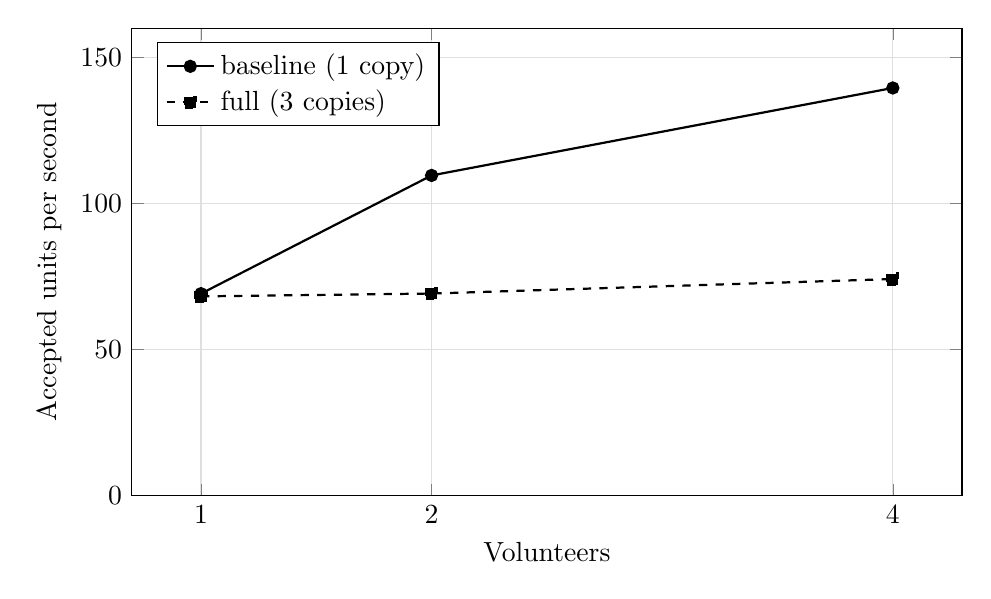
\begin{tikzpicture}
\begin{axis}[
  width=\columnwidth, height=0.62\columnwidth,
  xlabel={Volunteers}, ylabel={Accepted units per second},
  xtick={1,2,4}, ymin=0, ymax=160,
  legend pos=north west, legend cell align=left,
  grid=major, grid style={gray!25}]
\addplot[mark=*, thick] coordinates {(1,69.137) (2,109.607) (4,139.550)};
\addlegendentry{baseline (1 copy)}
\addplot[mark=square*, thick, dashed] coordinates {(1,68.207) (2,69.176) (4,74.142)};
\addlegendentry{full (3 copies)}
\end{axis}
\end{tikzpicture}
\caption{Throughput as volunteers are added, with 2 clients. Data: \texttt{results/load.csv}.}
\label{fig:load}
\end{figure}

\paragraph{More users}
With four volunteers in the full configuration, we vary the number of clients that submit jobs at the same time (Table~\ref{tab:clients}, Fig.~\ref{fig:clients}). With one client, the volunteers sit idle while a job is submitted, split and polled, so throughput is only 42.5 units per second. Two clients keep the volunteers busy, and throughput rises to 73.1. Beyond that it stays flat: the volunteers are the bottleneck, at about 75 units per second. Job time then grows with the number of clients, from a mean of 1.5\,s with one client to 4.7\,s with eight, as more jobs share the same volunteers; this is the expected queueing behavior. With eight clients, throughput falls slightly to 68.1 units per second, as more jobs and more polling compete for the single coordinator.

\begin{table}[t]
\centering
\caption{Throughput and job time with more clients (4 volunteers, full mode, 8 jobs)}
\label{tab:clients}
\begin{tabular}{@{}rrrrr@{}}
\toprule
Clients & Units/s & Jobs/min & Mean (s) & p95 (s) \\
\midrule
1 & 42.5 & 39.8 & 1.51 & 2.03 \\
2 & 73.1 & 68.5 & 1.64 & 2.25 \\
4 & 77.4 & 72.6 & 2.75 & 3.57 \\
8 & 68.1 & 63.9 & 4.66 & 7.52 \\
\bottomrule
\end{tabular}
\end{table}

\begin{figure}[t]
\centering
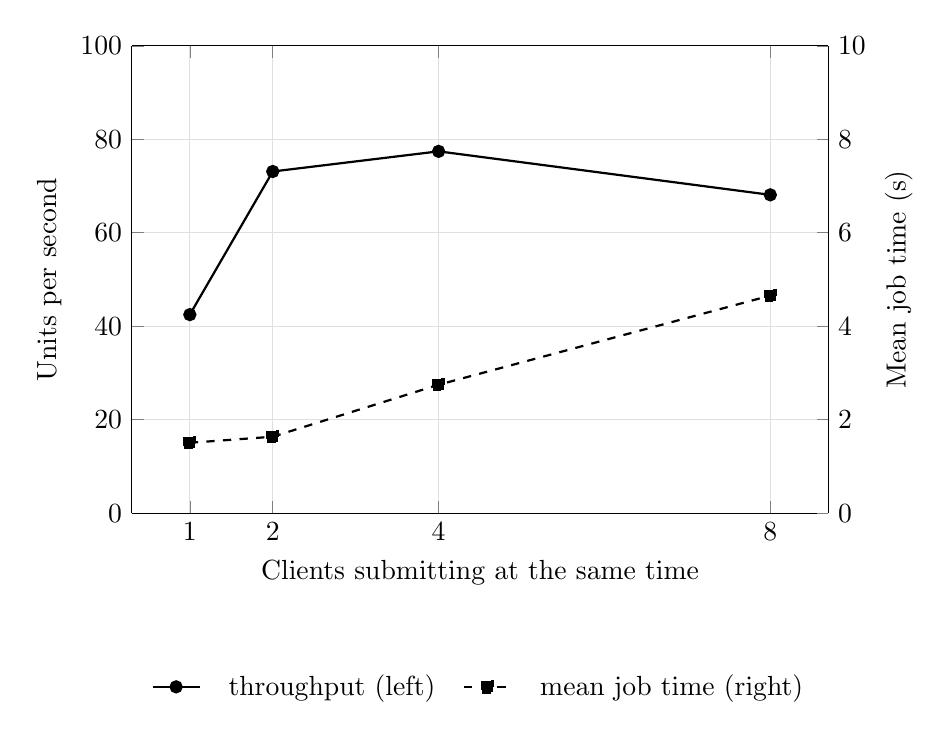
\begin{tikzpicture}
\begin{axis}[
  width=0.86\columnwidth, height=0.62\columnwidth,
  xlabel={Clients submitting at the same time}, ylabel={Units per second},
  xtick={1,2,4,8}, ymin=0, ymax=100,
  axis y line*=left,
  grid=major, grid style={gray!25}]
\addplot[mark=*, thick] coordinates {(1,42.489) (2,73.111) (4,77.420) (8,68.116)};
\end{axis}
\begin{axis}[
  width=0.86\columnwidth, height=0.62\columnwidth,
  xtick={1,2,4,8}, xticklabels={}, ymin=0, ymax=10,
  axis y line*=right, axis x line=none,
  ylabel={Mean job time (s)},
  legend style={at={(0.5,-0.32)}, anchor=north, legend columns=2, draw=none, column sep=8pt}]
\addlegendimage{mark=*, thick}
\addlegendentry{throughput (left)}
\addplot[mark=square*, thick, dashed] coordinates {(1,1.506) (2,1.637) (4,2.749) (8,4.656)};
\addlegendentry{mean job time (right)}
\end{axis}
\end{tikzpicture}
\caption{Throughput and job time as more users submit jobs (4 volunteers, full mode). Data: \texttt{results/load.csv}.}
\label{fig:clients}
\end{figure}
